%% Packages initialisation
\documentclass[10pt,compress]{beamer}
\usepackage[utf8]{inputenc}               % Enable UTF-8 compatible typing
\usepackage{hyperref}                     % Interactive PDF
\usepackage{tikz}
\usetikzlibrary{fit,calc,trees,positioning,arrows,chains,shapes.geometric,%
    decorations.pathreplacing,decorations.pathmorphing,shapes,%
    matrix,shapes.symbols,intersections}


%% Use the default theme
\usetheme{Madrid}

%% Colours block environment headings
\useinnertheme{rectangles}
\mode<beamer>{\setbeamertemplate{blocks}[rounded][shadow=false]} 
\setbeamercolor{block title}{bg=blue!10,fg=black}
\makeatletter
\pgfdeclareverticalshading[lower.bg,upper.bg]{bmb@transition}{200cm}{%
  color(0pt)=(upper.bg); color(2pt)=(upper.bg); color(4pt)=(upper.bg)}
\makeatother

%% Enable slide numbering
\makeatletter
\setbeamertemplate{footline}
{
  \leavevmode%
  \hbox{%
  \begin{beamercolorbox}[wd=.3\paperwidth,ht=2.25ex,dp=1ex,left]{author in head/foot}%
    \hspace*{2ex}\usebeamerfont{author in head/foot}\insertshortauthor~~\beamer@ifempty{\insertshortinstitute}{}{(\insertshortinstitute)}
  \end{beamercolorbox}%
  \begin{beamercolorbox}[wd=.5\paperwidth,ht=2.25ex,dp=1ex,center]{title in head/foot}%
    \usebeamerfont{title in head/foot}\insertshorttitle
  \end{beamercolorbox}%
  \begin{beamercolorbox}[wd=.2\paperwidth,ht=2.25ex,dp=1ex,right]{date in head/foot}%
    \usebeamerfont{date in head/foot} \usebeamerfont{date in head/foot}\insertshortdate{}\hfill \insertframenumber /\inserttotalframenumber\hspace*{2ex}
  \end{beamercolorbox}}%
  \vskip0pt%
}
\makeatother

%% Hide navigation buttons
\beamertemplatenavigationsymbolsempty

%% Listings
\usepackage{xcolor}
\usepackage{listings}

\lstset{
 backgroundcolor=\color{white},   % choose the background color; you must add \usepackage{color} or \usepackage{xcolor}
 basicstyle=\ttfamily\small,        % the size of the fonts that are used for the code
 commentstyle=\itshape,
 breakatwhitespace=false,         % sets if automatic breaks should only happen at whitespace
 breaklines=true,                 % sets automatic line breaking
 captionpos=b,                    % sets the caption-position to bottom
 deletekeywords={...},            % if you want to delete keywords from the given language
 escapeinside={§*}{*§},          % if you want to add LaTeX within your code
 extendedchars=true,              % lets you use non-ASCII characters; for 8-bits encodings only, does not work with UTF-8
 frame=none,	                   % adds a frame around the code
 keepspaces=true,                 % keeps spaces in text, useful for keeping indentation of code (possibly needs columns=flexible)
 numbers=none,                    % where to put the line-numbers; possible values are (none, left, right)
 rulecolor=\color{black},         % if not set, the frame-color may be changed on line-breaks within not-black text (e.g. comments (green here))
 showspaces=false,                % show spaces everywhere adding particular underscores; it overrides 'showstringspaces'
 showstringspaces=false,          % underline spaces within strings only
 showtabs=false,                  % show tabs within strings adding particular underscores
 tabsize=2,	                   % sets default tabsize to 2 spaces
 title=\lstname,                   % show the filename of files included with \lstinputlisting; also try caption instead of title
  belowcaptionskip=-1\baselineskip,
  xleftmargin=\parindent
}

\definecolor{darkgreen}{rgb}{0.000000,0.392157,0.000000}
\definecolor{violetred}{rgb}{0.915686,0.125490,0.364706}

% Define Links as a lst-language
\lstdefinelanguage{Links}{% 
  morekeywords={spawn, receive, typename, fun, op, var, if, this, true, false, else, case, switch, handle, handler, shallowhandler, do, sig, spawnAngel, spawnDemon, spawn},%
  sensitive=t, % 
  keywordstyle=\color{red},
  emph={Comp,Player,Bool,Int,GTree,Cheat,Zero,Choose,Rand,Move,Winner,Take,Return,Get,Put,GameState,Alice,Bob,Fail,Nothing,Just,Maybe,Toss,Heads,Tails,Process,Buyer,Coffee,Pay,Cost,Candidate,Stop,PassingComet,CelebritySighting,Float,String,Pid,EProcess,Row,Spawn,Yield,Recv,Send,FreshName,Queue,Dictionary,Myself,Type},
  emphstyle={\color{blue}},
  comment=[l]{\#},% 
  commentstyle={\itshape\color{darkgreen}},%
  escapeinside={(*}{*)},%
  morestring=[d]{"},%
  stringstyle={\color{violetred}}%
 }

% Haskell style
\lstdefinestyle{haskell}{
  language=Haskell,
  basicstyle=\linespread{1.0}\ttfamily\footnotesize,
  literate= {+}{{$+$}}1 {*}{{$*$}}1
            {<=}{{$\leq$}}1 {/=}{{$\neq$}}1 
            {==}{{$\equiv$}}1 {=>}{{$\Rightarrow$}}1
            {->}{{$\to$}}1 {<-}{{$\leftarrow$}}1
            {.}{{$\circ$}}1 {$$}{{\$}}1
}
% Ocaml style
\lstdefinestyle{ocaml}{
  language=Caml,%
  morekeywords={effect, perform},%
  emph={Obj,Choose},%
%  literate= {+}{{$+$}}1 {*}{{$*$}}1
%            {<=}{{$\leq$}}1 {>=}{{$\geq$}}1 {<>}{{$\neq$}}1 
%            {==}{{$\equiv$}}1 {=>}{{$\Rightarrow$}}1
%            {->}{{$\to$}}1
}

\usepackage{textcomp}
%\newcommand{\textapprox}{{\fontfamily{ptm}\selectfont\texttildelow}}
%\newcommand{\wildarrow}{\linksify{\textapprox{}>}}
\newcommand{\wildarrow}{\fontfamily{ptm}\selectfont\linksify{\textasciitilde{}>}}
% Links style
\lstdefinestyle{links}{
  caption={},
  basicstyle=\linespread{1.0}\ttfamily\footnotesize,
  language=Links,
  literate= {~>}{{\wildarrow}}1
}

\lstset{style={links}}

% Terminal / prompt style
\lstdefinestyle{terminal}{
  caption={},
  basicstyle=\linespread{1.0}\ttfamily\footnotesize,
  keywordstyle={},
  emphstyle={},
  commentstyle={}
}

%% Meta information
\author[D. Hillerström]{Daniel Hillerström \inst{1} \and Sam Lindley \inst{1} \and KC Sivaramakrishnan \inst{2}}
\title{Compiling Links Effect Handlers to the OCaml Backend}
\institute[University of Edinburgh]{\inst{1} The University of Edinburgh, UK \and \inst{2} University of Cambridge, UK}
\subtitle{ML Workshop '16}
\date[22-09-2016]{September 22, 2016}

%% Slides
\begin{document}
% Sponsors slide
\begin{frame}[plain]
\frametitle{This work is supported by}
\begin{columns}[T]
\begin{column}{0.5\textwidth}
\begin{figure}

\includegraphics[scale=0.6]{figures/uoe.eps}
\end{figure}
\end{column}
\hfill
\begin{column}{0.5\textwidth}
\begin{figure}

\includegraphics[scale=0.6]{figures/school_of_informatics.eps}
\end{figure}
\end{column}
\end{columns}

\vfill

\begin{columns}[T]
\begin{column}{0.5\textwidth}
\begin{figure}

\includegraphics[scale=0.35]{figures/cdtppar.eps}
\end{figure}
\end{column}
\hfill
\begin{column}{0.5\textwidth}
\begin{figure}

\includegraphics[scale=0.3]{figures/epsrc.eps}
\end{figure}
\end{column}
\end{columns}

\vfill

\begin{columns}[T]
\begin{column}{0.5\textwidth}
\begin{figure}

\includegraphics[scale=0.18]{figures/cambridge.eps}
\end{figure}
\end{column}
\hfill
\begin{column}{0.5\textwidth}
\begin{figure}
OCaml Labs
\end{figure}
\end{column}
\end{columns}

\end{frame}

% Title slide
\begin{frame}[plain]
  \maketitle
\end{frame}

%% Introduction of Links
\begin{frame}
\frametitle{The Programming Language Links}
Meet Links
\begin{itemize}
  \item a ML-like strict functional programming language,
  \item a single-source language for multi-tier web-programming,
  \item with a syntax reminiscent of JavaScript, e.g. \lstinline$fun foo(x,y) \{ ... \}$,
  \item and a strong type system including linear types,
  \item with effect typing based on row polymorphism,
  \item and it provides \emph{effect handlers} for controlling effects.
\end{itemize}
Links has three backends, each written in OCaml:
\begin{itemize}
 \item a JavaScript compiler for the client,
 \item an interpreter for the server,
 \item and an SQL generator for the database,
 \item and with this work a compiler for the server.
\end{itemize}
See more at \url{http://www.links-lang.org}.
\end{frame}

%% Introduction of handlers
\begin{frame}[fragile]
\frametitle{Algebraic Effects and Abstract Computations}
An algebraic effect is a collection of \emph{abstract operations}, e.g.

\[ 
Nondet = \{\text{\lstinline$Choose : Bool$}\}, \qquad Failure = \{\text{\lstinline$Fail : Zero$}\}
\]

Using these operations we can define effectful computations \emph{abstractly}, e.g.
\begin{onlyenv}<1-1>
\begin{lstlisting}

fun toss() { if (do Choose) Heads else Tails }
\end{lstlisting}
\end{onlyenv}
%
\begin{onlyenv}<2-2>
\begin{lstlisting}

fun toss() { if (choose()) Heads else Tails }
\end{lstlisting}
\end{onlyenv}
%
\begin{onlyenv}<3-4>
\begin{lstlisting}
sig toss : () {Choose:Bool|e}-> Toss
fun toss() { if (choose()) Heads else Tails }
\end{lstlisting}
\end{onlyenv}
%

Algebraic effects compose seamlessly, e.g.
\begin{onlyenv}<1-1>
\begin{lstlisting}

fun drunkToss() { if (do Choose) toss() else switch (do Fail) { } }
\end{lstlisting}
\end{onlyenv}
%
\begin{onlyenv}<2-2>
\begin{lstlisting}

fun drunkToss() { if (choose()) toss() else fail() }
\end{lstlisting}
\end{onlyenv}
%
\begin{onlyenv}<3-4>
\begin{lstlisting}
sig drunkToss : () {Choose:Bool,Fail:Zero|e}-> Toss
fun drunkToss() { if (choose()) toss() else fail() }
\end{lstlisting}
\end{onlyenv}

\begin{uncoverenv}<4-4>
Evaluation of an abstract computation\dots
\begin{lstlisting}[style=terminal]
links> drunkToss();
*** Error: Unhandled operation: Choose
\end{lstlisting}
\dots but, what are the semantics of \lstinline$Choose$ and \lstinline$Fail$?
\end{uncoverenv}

\end{frame}

\begin{frame}[fragile]
  \frametitle{Abstract Operation Instantiation with Affine Handlers} 
%
  A handler instantiates abstract operations with concrete
  implementations, e.g.
%% Random result animation
\begin{onlyenv}<1-1>
\begin{lstlisting}


handler randomResult {
  case Return(x) -> x
  case Choose(resume) -> resume(random() > 0.5)
}
\end{lstlisting}
\end{onlyenv}
%
\begin{onlyenv}<2-3>
\begin{lstlisting}
sig randomResult : (() {Choose:Bool|e}-> a) -> 
                    () {Choose{_}  |e}-> a
handler randomResult {
  case Return(x) -> x
  case Choose(resume) -> resume(random() > 0.5)
}
\end{lstlisting}
\end{onlyenv}
%
%% All results animation
\begin{onlyenv}<4-5>
\begin{lstlisting}
sig allResults : (() {Choose:Bool|e}->  a) -> 
                  () {Choose{_}  |e}-> [a]
handler allResults {
  case Return(x) -> [x]
  case Choose(resume) -> resume(true) ++ resume(false)
}
\end{lstlisting}
\end{onlyenv}
%
The function \lstinline$resume$ is the captured (delimited) continuation of the operation.
\vfill
\begin{onlyenv}<3-4>
Interpretation of \lstinline$toss$ with this handler:
\begin{onlyenv}<3-3>
\begin{lstlisting}[style=terminal]
links> randomResult(toss)();
Tails : Toss
\end{lstlisting}
\end{onlyenv}
%
\begin{onlyenv}<4-4>
\begin{lstlisting}[style=terminal]
links> allResults(toss)();
[Heads, Tails] : [Toss]
\end{lstlisting}
\end{onlyenv}
\end{onlyenv}

\begin{onlyenv}<5-5>
Interpretation of \lstinline$drunkToss$ with either handler:
\begin{lstlisting}[style=terminal]
links> allResults(drunkToss)();
*** Error: Unhandled operation: Fail
\end{lstlisting}
\end{onlyenv}
\end{frame}

\begin{frame}[fragile]
\frametitle{Exception Handling}
%
We can define a handler for \lstinline$Fail$ independently, e.g.
%
\begin{lstlisting}
sig maybeResult : (() {Fail:Zero|e}->       a) ->
                   () {Fail{_}  |e}-> Maybe(a)
handler maybeResult {
  case Return(x) -> Just(x)
  case Fail(_)   -> Nothing
}
\end{lstlisting}
%
Impossible to invoke the continuation because \lstinline$Fail$ expects
a value of \lstinline$Zero$. Thus, this handler amounts to an \emph{exception handler}.
\vfill
Handlers compose to fully interpret an abstract computation, e.g.
\begin{onlyenv}<1-1>
\begin{lstlisting}[style=terminal]
links> maybeResult(allResults(drunkToss))();
Just([Heads, Tails]) : Maybe([Toss])
\end{lstlisting}
\end{onlyenv}
%
\begin{onlyenv}<2-2>
\begin{lstlisting}[style=terminal]
links> allResults(maybeResult(drunkToss))();
[Just(Heads), Just(Tails), Nothing] : [Maybe(Toss)]
\end{lstlisting}
\end{onlyenv}
\end{frame}

\begin{frame}[fragile]
  \frametitle{Classification of Handlers}
Exception handlers
\hrule
\begin{columns}
\begin{column}{0.6\textwidth}
\begin{lstlisting}
handler maybeResult {
  case Return(x) -> Just(x)
  case Fail(_)   -> Nothing
}
\end{lstlisting}
\end{column}
\hfill
\begin{column}{0.4\textwidth}
Zero invocations of the continuation.
\end{column}
\end{columns}
%

Linear handlers
\hrule
\begin{columns}
\begin{column}{0.6\textwidth}
\begin{lstlisting}
handler randomResult {
  case Return(x)      -> x
  case Choose(resume) -> 
     resume(random() > 0.5)
}
\end{lstlisting}
\end{column}
\hfill
\begin{column}{0.4\textwidth}
Linear consumption of the continuation.
\end{column}
\end{columns}

Multi-shot handlers
\hrule
\begin{columns}
\begin{column}{0.6\textwidth}
\begin{lstlisting}
handler allResults {
  case Return(x)      -> [x]
  case Choose(resume) -> 
     resume(true) ++ resume(false)
}
\end{lstlisting}
\end{column}
\hfill
\begin{column}{0.4\textwidth}
Multiple consumptions of the continuation.
\end{column}
\end{columns}
Exception and linear handlers are also known as \emph{affine} handlers.
\end{frame}

%% Compiling handlers
\begin{frame}
  \frametitle{Aim}
Want to make this abstraction efficient.
\end{frame}

\begin{frame}
  \frametitle{Compiling Handlers}
Compilation options
\begin{itemize}
  \item Free monad (Bauer and Pretnar, 2015)
  \item Continuation monad (Kammar et al., 2013)
  \item Full CPS translation
  \item Selective CPS translation (Leijen, 2016)
  \item \alt<2>{\tikz[baseline,remember picture]{\node[fill=green!20,anchor=base,rounded corners=2pt] (t1){Direct-style like Multicore OCaml (Dolan et al., 2015).};}}{Direct-style like Multicore OCaml (Dolan et al., 2015).}
\end{itemize}
\end{frame}

%% Compiler backend overview
\begin{frame}[fragile]
  \frametitle{Compiler Backend}
\begin{figure}
\tikzset{my rectangle/.style={
        draw=black,
        thick, 
        rectangle, 
        minimum width={width("OCaml frontend")+2pt}}
}
\centering
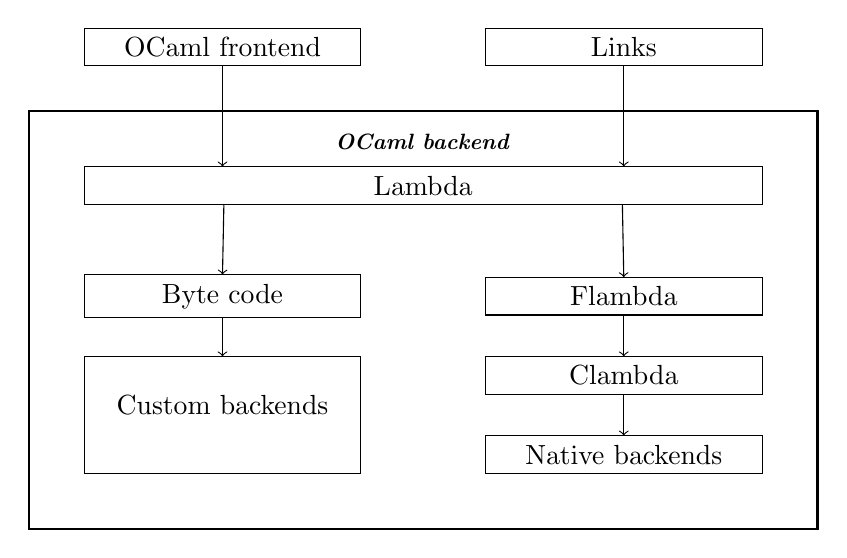
\begin{tikzpicture}[node distance=5pt,every node/.style={draw, minimum width=100pt, outer sep=0pt}]

  \node(A)          {OCaml frontend};
  \node(B)[right=of A,xshift=40pt] {Links};

  \node(C)[inner sep=0pt,yshift=-50pt,fit={(A) (B)},label=center:Lambda] {};

  \node[above=of C,draw=none,yshift=-2pt] {\footnotesize{\textbf{\textit{OCaml backend}}}};

  \node(D)[yshift=-90pt]          {Byte code};
  \node(E)[right=of D,xshift=40pt] {Flambda};

  \node(G)[below=of E,yshift=-10pt] {Clambda};
  \node(H)[below=of G,yshift=-10pt] {Native backends};

  \node(F)[fit=(G)(H),inner sep=0,left=of G.north west,anchor=north east,xshift=-40pt]          {Custom backends};


  \node(Z)[thick,fit=(C)(H),inner sep=20pt] {};

  \draw[->] (A.south) to ([xshift=50pt]C.north west);
  \draw[->] (B.south) to ([xshift=-50pt]C.north east);

  \draw[->] ([xshift=-72pt]C.south) to (D.north);

  \draw[->] (D) to (F);

  \draw[->] ([xshift=72pt]C.south) to (E.north);
  \draw[->] (E) to (G);
  \draw[->] (G) to (H);
%  \node(C)[below=of B] {C};
%  \node(D)[below=of C] {D};

%  \node(Z)[fit=(A)(D),right=of A.north east,anchor=north west, inner sep=0] {Z};

% % Frontends
% \node [my rectangle] (OCaml frontend) at (0,0) {OCaml frontend};
% \node [my rectangle] (Links frontend) at (6,0) {Links frontend};

% % OCaml backend
% \node [my rectangle,minimum width=270pt] (Lambda) at (3,-2) {Lambda};
% %\node[rectangle,draw=black,ultra thick,minimum height=+5.0cm,minimum width=+4.0cm,fit ={(Parser.north) (Typechecker.south)}] (Frontend) {};
\end{tikzpicture}
\end{figure}
\end{frame}

\begin{frame}
  \frametitle{Multicore OCaml Handlers}
%
Multicore OCaml
\begin{itemize}
\item provides effect handlers as abstraction for concurrency,
\item provides an efficient, native implementation of affine effect handlers,
\item and implements handlers as heap-managed stack data structures.
\end{itemize}
Runtime layout of \lstinline$randomResult(maybeResult(drunkToss))$:
\begin{figure}
\tikzset{stack/.style={
        draw=black, 
        rectangle, 
        minimum width=18pt,
        minimum height=55pt,
        fill=blue!75}
}

\tikzset{handler/.style={
        draw=black, 
        rectangle, 
        minimum width=18pt,
        minimum height=15pt,
        fill=green!75}
}
\begin{tikzpicture}[node distance=0pt,every node/.style={draw, rectangle,  minimum width=10pt, outer sep=0pt}]

\node [stack] (s1) { };
\node [handler,above=of s1] (h1) { $H_1$ };
\node [draw=none,below=of s1,yshift=-20pt] (oplabel) { Handles \lstinline$Choose$ };

\node [draw=none,left=of h1,xshift=-20pt,yshift=-10pt] (h1label) {handler};

\node [stack,right=of s1,xshift=70pt] (s2) { };
\node [handler,above=of s2] (h2) { $H_2$ };

\node [stack,right=of s2,xshift=70pt] (s3) { };

\node [draw=none,below=of s3,yshift=-20pt] (drunkToss) { \lstinline$drunkToss$ computation };

\node [draw=none,above=of s3,yshift=25pt] (ghost1) { };
\node [draw=none,right=of ghost1,xshift=15pt] (ghost2) { call chain };
\node [draw=none,above=of ghost1,yshift=5pt] (ghost3) { };
\node [draw=none,right=of ghost3,xshift=15pt] (ghost4) { reference };
\draw[dotted,thick,->] (ghost1) -- (ghost2) { };
\draw[thick,->] (ghost3) -- (ghost4) { };

\uncover<2-2>{\node [draw=none,left=of s3,yshift=30pt,xshift=-5pt] {\lstinline$do Choose$};}
\uncover<5-5>{\node [draw=none,left=of s3,yshift=30pt,xshift=5pt] {\lstinline$resume(true)$};}
\uncover<2-5>{\draw[thick,->] (h2) -- (s3) { };}

\uncover<3-3>{\node [draw=none,left=of h2,xshift=-2pt,yshift=6pt] {forward \lstinline$Choose$};}
\uncover<4-4>{\node [draw=none,left=of h2,xshift=-2pt,yshift=6pt] {\lstinline$resume(true)$};}
\uncover<3-4>{\draw[thick,->] (h1) -- (h2) { };}

% Arrows
\draw[->,thick] ([yshift=-10pt]s2.west) -- ([yshift=-10pt]s1.east) { };
\draw[dotted,thick,->] (h1.east) [in=180,out=0] to ([yshift=2pt]s2.south west) { };
\draw[->] (h1label.east) -- (h1.west) { };

\draw[->,thick] ([yshift=-10pt]s3.west) -- ([yshift=-10pt]s2.east) { };
\draw[dotted,thick,->] (h2.east) [in=180,out=0] to ([yshift=2pt]s3.south west) { };

\draw[->,draw=red!90,thick] (oplabel) [in=-95,out=80] to (h1) { };
\draw[->,draw=red!90,thick] (drunkToss) [in=-95,out=80] to (s3.south) { };
\end{tikzpicture}
\end{figure}
\end{frame}

\begin{frame}
  Todo
\begin{itemize}
  \item Motivation for handlers
  \item OCaml provides efficient implementation of handlers (show stack diagram)
  \item From nice ideal world, to practical and efficient world (type-directed).
  \item Report on optimisations
  \item Sometime we do not want linear continuation to be promoted.
\end{itemize}
\end{frame}

\begin{frame}
  \frametitle{Summary}
\begin{itemize}
\item Algebraic effects and handlers provide a modular abstraction for
  effectful programming.
\item Regard Links as an experimental frontend to OCaml with effect
  typing and linear types.
\item Type-directed optimisation of effect handlers\dots
\end{itemize}
\end{frame}

% Load subsequent slides, e.g.
%\input{slides/index}

% Bibliography
\bibliographystyle{unsrt}
\begin{frame}[allowframebreaks]
  \frametitle{References}
  \nocite{*}
  \bibliography{compilinghandlers}
\end{frame}
\end{document}
